\documentclass{article}
\usepackage{tikz}

\begin{document}
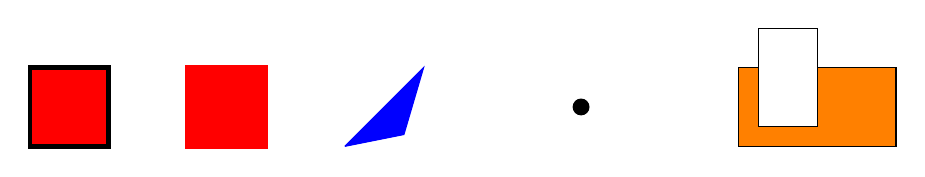
\begin{tikzpicture}
\draw [fill=red,ultra thick] (0,0) rectangle (1,1);
\draw [fill=red,ultra thick,red] (2,0) rectangle (3,1);
\draw [blue, fill=blue] (4,0) -- (5,1) -- (4.75,0.15) -- (4,0);
\draw [fill] (7,0.5) circle [radius=0.1];
\draw [fill=orange] (9,0) rectangle (11,1);
\draw [fill=white] (9.25,0.25) rectangle (10,1.5);
\end{tikzpicture}


\begin{tikzpicture}
\path [fill=yellow] (0,0) rectangle (1.5,1);
\draw [fill=yellow] (2,0) rectangle (3.5,1);
\end{tikzpicture}


\begin{tikzpicture}
\draw [ultra thick] (0,0) to [out=87, in=150] (1,1)--(.85,.15)--(0,0);
\draw [ultra thick,fill=purple] (2,0) to [out=87, in=150] (3,1) -- (2.85,.15) --(2,0);
\path [fill=purple] (4,0) to [out=87, in=150] (5,1) -- (4.85,.15) --(4,0);
\end{tikzpicture}

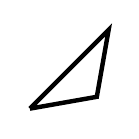
\begin{tikzpicture}
\draw [ultra thick] (0,0) to (1,1) to (.85,.15) to (0,0);
\end{tikzpicture}

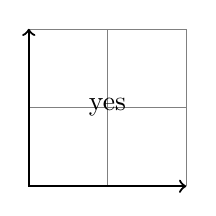
\begin{tikzpicture}
\draw[help lines] (0,0) grid (2,2);
\draw [thick,<->] (0,2) -- (0,0) --(2,0);
\node at (1,1) {yes};
\end{tikzpicture}

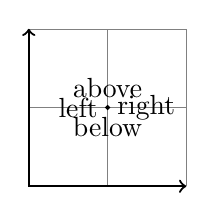
\begin{tikzpicture}
\draw[help lines] (0,0) grid (2,2);
\draw [thick,<->] (0,2) -- (0,0) --(2,0);
\draw [fill] (1,1) circle [radius=0.025];
\node [below] at (1,1) {below};
\node [above] at (1,1) {above};
\node [left] at (1,1) {left};
\node [right] at (1,1) {right};
\end{tikzpicture}

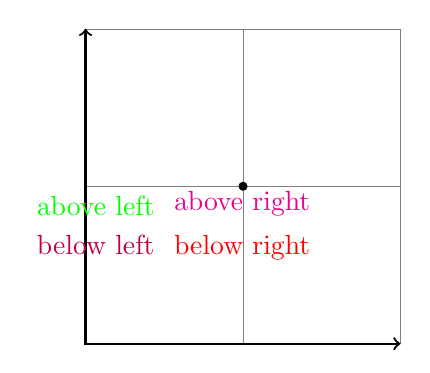
\begin{tikzpicture}[scale=2]
\draw[help lines] (0,0) grid (2,2);
\draw [thick, <->] (0,2) -- (0,0) -- (2,0);
\draw[fill] (1,1) circle [radius=0.025];
\node [below right, red] at (.5,.75) {below right};
\node [above left, green] at (.5,.75) {above left};
\node [below left, purple] at (.5,.75) {below left};
\node [above right, magenta] at (.5,.75) {above right};
\end{tikzpicture}\\\\\\

\begin{tikzpicture}[xscale=3, yscale=1.5]
\draw[help lines] (0,0) grid (2,2);
\draw [thick, <->] (0,1) -- (0,0) -- (1,0);
\node [below right] at (1,0) {$x$};
\node [left] at (0,1) {$y$};
\draw [fill] (0.4,0.6) circle  [radius=0.5pt];
\node [above right] at (0.4,0.6) {$A$};
\end{tikzpicture}

\begin{tikzpicture}[xscale=3, yscale=3]
\draw [thick, <->] (0,1) node [left]  {$y$} -- (0,0) -- (1,0) node [below right] {$x$};
\draw [fill] (.4,.6) circle  [radius=.5pt] node[above right] (.4,.6) {$A$};
\end{tikzpicture}

\begin{tikzpicture}
\end{tikzpicture}
\end{document}